% Created 2019-02-25 Mon 14:11
\documentclass[11pt]{article}
\usepackage[utf8]{inputenc}
\usepackage[T1]{fontenc}
\usepackage{fixltx2e}
\usepackage{graphicx}
\usepackage{longtable}
\usepackage{float}
\usepackage{wrapfig}
\usepackage{rotating}
\usepackage[normalem]{ulem}
\usepackage{amsmath}
\usepackage{textcomp}
\usepackage{marvosym}
\usepackage{wasysym}
\usepackage{amssymb}
\usepackage{hyperref}
\tolerance=1000
\usepackage{minted}
\usepackage{amsthm}
\usepackage[margin=1.0in]{geometry}
\setlength{\parindent}{0pt}
\setlength{\parskip}{\baselineskip}
\author{Thomas Alford}
\date{\today}
\title{Ph21 Problem Set 4}
\hypersetup{
  pdfkeywords={},
  pdfsubject={},
  pdfcreator={Emacs 25.2.1 (Org mode 8.2.10)}}
\begin{document}

\maketitle
\section*{Problem 1}
\label{sec-1}
\subsection*{Imports}
\label{sec-1-1}
\begin{minted}[frame=lines,fontsize=\scriptsize]{python}
import numpy as np
import matplotlib.pyplot as plt
%matplotlib inline
\end{minted}

\subsection*{Coin Tossing in Numpy}
\label{sec-1-2}
\begin{minted}[frame=lines,fontsize=\scriptsize]{python}
def biased_flip(H, size=None):
    return np.random.random(size=size) < H
\end{minted}


Here we will get data on the number of heads in n tosses for each value of
n. Then, go through a grid of values for H and calculate how likely they was
given the data. Then mult this by the prior for each value to get post

\begin{minted}[frame=lines,fontsize=\scriptsize]{python}
def get_H_vals(H):
    nvals = [2 ** n for n in range(8)]
    ntrials = 1

    bflips = [biased_flip(H, size=[ntrials, n]) for n in nvals]
    sums = np.array(list(map(np.sum, bflips)))
    return sums, nvals
\end{minted}


\begin{minted}[frame=lines,fontsize=\scriptsize]{python}
sums, nvals = get_H_vals(.5)
\end{minted}

\subsection*{Likelihood}
\label{sec-1-3}
Now we need to get the probability of each amount given some values of H:

\begin{minted}[frame=lines,fontsize=\scriptsize]{python}
def get_H_prob(n, h, H):
    return (np.math.factorial(n) / (np.math.factorial(h) * np.math.factorial(
        n - h))) * H ** h * (1 - H) ** (n - h)
\end{minted}


\begin{minted}[frame=lines,fontsize=\scriptsize]{python}
H_vals = np.linspace(0, 1, 20)
H_probs = [[get_H_prob(nvals[i], sums[i], H) for H in H_vals] for i in range(
    len(nvals))]
\end{minted}
\subsection*{Plotting Posteriors}
\label{sec-1-4}

\begin{minted}[frame=lines,fontsize=\scriptsize]{python}
def plot_H_probs(real_H, H_vals, H_probs, prior_func, **prior_kwargs):
    fig, axes = plt.subplots(4, 2, figsize=(8, 7))
    for i, val in enumerate(nvals):
        ax = axes.flatten()[i]
        ax.plot(H_vals, H_probs[i], label='n=%s'%val)
        prior_vals = np.array([prior_func(H, **prior_kwargs) for H in H_vals])
        normed_vals = prior_vals * (np.max(H_probs[i]) / np.max(prior_vals))
        ax.plot(H_vals, normed_vals, '--', label='prior')
        ax.legend()

    plt.suptitle('Posterior probabilities of H with real H = %s' %real_H)
    fig.text(0.5, 0.04, 'Number of Heads', ha='center')
    fig.text(0.04, 0.5, 'Posterior Density', va='center', rotation='vertical')
    plt.subplots_adjust(top=0.9, hspace=.6)
    plt.show()

def get_and_plot_H(H, prior_func, **prior_kwargs):
    sums, nvals = get_H_vals(H)
    H_vals = np.linspace(0, 1, 20)
    H_probs = [[get_H_prob(nvals[i], sums[i], H) * prior_func(
        H, **prior_kwargs) for H in H_vals] for i in range(len(nvals))]
    plot_H_probs(H, H_vals, H_probs, prior_func, **prior_kwargs)
    
def uniform_prior(H):
    return 1
\end{minted}

\subsubsection*{Uniform Priors}
\label{sec-1-4-1}

\begin{minted}[frame=lines,fontsize=\scriptsize]{python}
get_and_plot_H(.5, uniform_prior)
\end{minted}

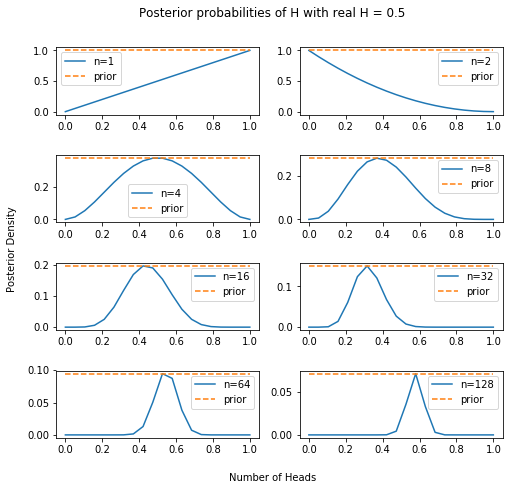
\includegraphics[width=.9\linewidth]{./obipy-resources/3223KS.png}

Now let's try doing this for different values of H:

\begin{minted}[frame=lines,fontsize=\scriptsize]{python}
get_and_plot_H(.6, uniform_prior)
\end{minted}

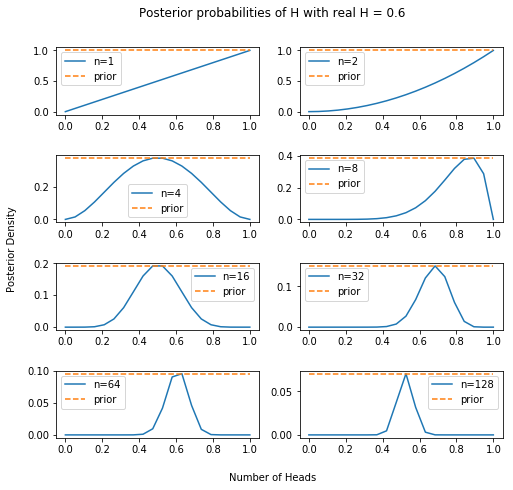
\includegraphics[width=.9\linewidth]{./obipy-resources/322EVY.png}

\begin{minted}[frame=lines,fontsize=\scriptsize]{python}
get_and_plot_H(.8, uniform_prior)
\end{minted}

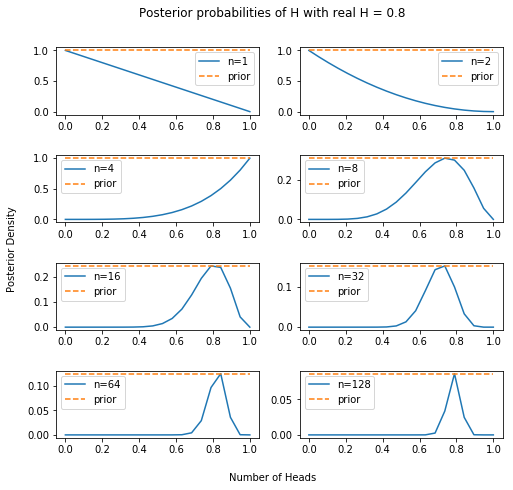
\includegraphics[width=.9\linewidth]{./obipy-resources/322Rfe.png}

These 'posteriors' were actually the same as our data, or 'likelihood' plots,
as our prior was uniform.

Now we can start working non-uniform priors:

Here we'll just multiply all of our 'likelihood' values by their prior
probabilities. First, we'll start our using a Gaussian prior with mean at .5,
and standard devition of 1.

\subsubsection*{Gaussian Priors}
\label{sec-1-4-2}

\begin{minted}[frame=lines,fontsize=\scriptsize]{python}
def gaussian(x, mu=0, sigma=1, C=1):
    return C * np.exp((-(x - mu) ** 2) / (2 * sigma ** 2))

plt.plot(np.linspace(-3, 3, 100), gaussian(np.linspace(-3, 3, 100),
                                           mu=.5, sigma=.5))
plt.xlim([-2.5, 3])
plt.title('Gaussian Function')
plt.show()
\end{minted}

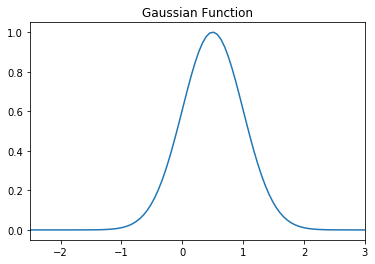
\includegraphics[width=.9\linewidth]{./obipy-resources/322EcM.png}

\begin{minted}[frame=lines,fontsize=\scriptsize]{python}
get_and_plot_H(.5, gaussian, mu=.5, sigma=.25)
\end{minted}

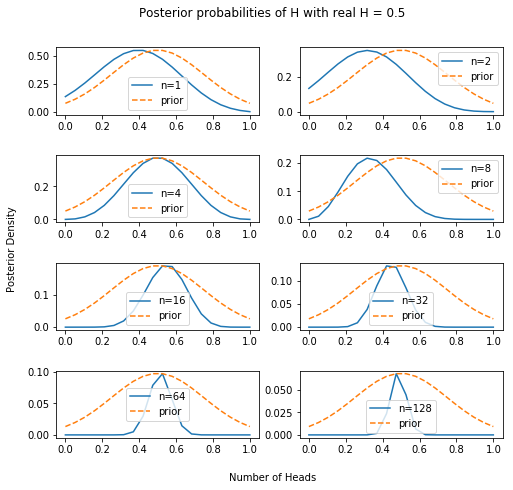
\includegraphics[width=.9\linewidth]{./obipy-resources/322rzq.png}

\begin{minted}[frame=lines,fontsize=\scriptsize]{python}
get_and_plot_H(.7, gaussian, mu=.5, sigma=.25)
\end{minted}

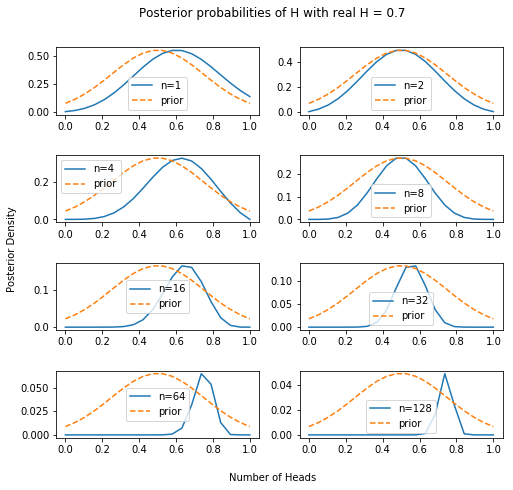
\includegraphics[width=.9\linewidth]{./obipy-resources/32249w.png}

\begin{minted}[frame=lines,fontsize=\scriptsize]{python}
get_and_plot_H(.7, gaussian, mu=.3, sigma=.1)
\end{minted}

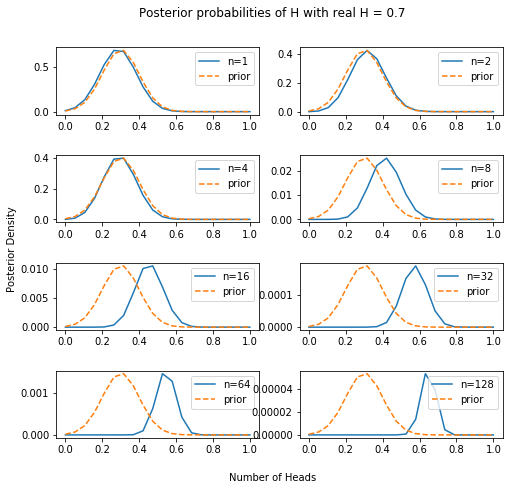
\includegraphics[width=.9\linewidth]{./obipy-resources/3223RG.png}

Here even though the prior is over 3 sigma away, we see that as the trials
increase our posterior still peaks pretty close to the correct value of H.

\section*{Problem 2}
\label{sec-2}
Here let's try simulating the lighthouse flash at many random angles, seeing
where they end up on shore. 

Here we need the probability that an angle landed at a given location given
alpha and beta. If we look at specific locations, that probability will
actually be zero. However, if we round to the nearest 2 decimal places, for
instance, we'll be able to integrate to get the probability for each.

\subsection*{Getting random angles}
\label{sec-2-1}

\begin{minted}[frame=lines,fontsize=\scriptsize]{python}
def rand_angle(size=None):
    return np.random.random(size=size) * np.pi - np.pi / 2
\end{minted}

\subsection*{Getting the likelihood}
\label{sec-2-2}

\begin{minted}[frame=lines,fontsize=\scriptsize]{python}
def get_theta(d, alpha, beta):
    return np.arctan((d - alpha) / beta)

def get_prob(d, alpha, beta):
    # assume d has been rounded to two places i.e. 1.22
    # range is then 1.215 to 1.225
    high_bound = get_theta(d + .005, alpha, beta)
    low_bound = get_theta(d - .005, alpha, beta)
    diff = np.abs(high_bound - low_bound)
    # this is basically our unnormalized probability
    return diff
\end{minted}


\begin{minted}[frame=lines,fontsize=\scriptsize]{python}
plt.plot(np.linspace(-10, 10, 100), [get_prob(x, 0, 1) for x in np.linspace(
    -10, 10, 100)])
\end{minted}

\begin{verbatim}
[<matplotlib.lines.Line2D at 0x119d39198>]
\end{verbatim}
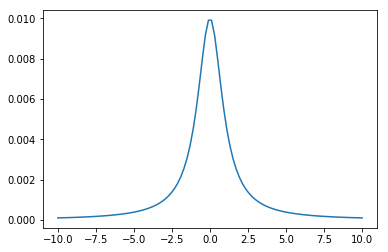
\includegraphics[width=.9\linewidth]{./obipy-resources/322RmS.png}

Here it looks like this works. Now let's get some actual data and get posterior
probabilities based on a uniform prior:

\begin{minted}[frame=lines,fontsize=\scriptsize]{python}
def get_rand_locs(nlocs, alpha, beta):
    angles = rand_angle(size=nlocs)
    # have that alpha - loc = beta * tan(theta)
    diff = beta * np.tan(angles)
    loc = alpha - diff
    return loc
\end{minted}


\begin{minted}[frame=lines,fontsize=\scriptsize]{python}
def plot_locs(alpha, beta, n, ax):
    locs = get_rand_locs(n, alpha, beta)
    # round locations
    locs = np.round(locs, decimals=2)
    ax.hist(locs, bins=n, density=True, label='n=%s'%n)
    ax.set_xlim(-50, 50)
    ax.legend()
    #ax.set_xlabel('location')
    #plt.ylabel('density')
    #plt.title('Locations for alpha=%s, beta=%s'%(alpha, beta))
    return locs
\end{minted}


\begin{minted}[frame=lines,fontsize=\scriptsize]{python}
def plot_dists(alpha, beta):
    fig, axes = plt.subplots(4, 2, figsize=(8, 7))
    means = []
    for i, n in enumerate(nvals):
        locs = plot_locs(alpha, beta, n, axes.flatten()[i])
        means.append(np.mean(locs))

    plt.suptitle('Distributions of {x_k} for alpha=%s, beta=%s'%(alpha, beta))
    fig.text(0.5, 0.04, 'Location', ha='center')
    fig.text(0.04, 0.5, 'Density', va='center', rotation='vertical')
    plt.subplots_adjust(top=0.9, hspace=.6)
    plt.show()
    return means
\end{minted}

\subsubsection*{Original \{x$_{\text{k}}$\} Distributions}
\label{sec-2-2-1}

\begin{minted}[frame=lines,fontsize=\scriptsize]{python}
means = plot_dists(0, 2)
\end{minted}

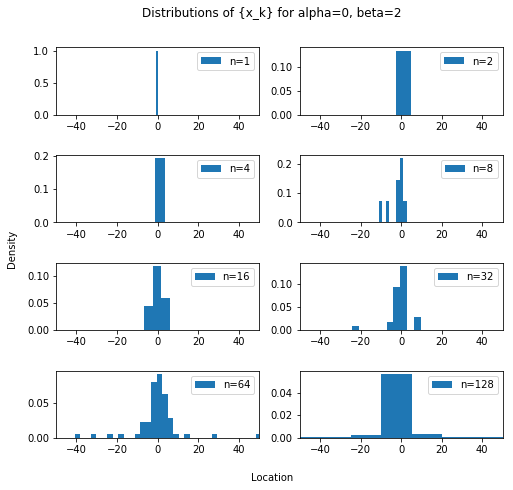
\includegraphics[width=.9\linewidth]{./obipy-resources/322i7o.png}

\begin{minted}[frame=lines,fontsize=\scriptsize]{python}
for i, mean in enumerate(means):
    print('n=%s, mean=%s'%(nvals[i], mean))
\end{minted}

\begin{verbatim}
n=1, mean=-0.21
n=2, mean=1.2349999999999999
n=4, mean=1.42
n=8, mean=-1.99125
n=16, mean=-3.6450000000000005
n=32, mean=-3.6715625
n=64, mean=1.8871874999999996
n=128, mean=8.888203125000004
\end{verbatim}


\begin{minted}[frame=lines,fontsize=\scriptsize]{python}
new_means = plot_dists(2, 4)
\end{minted}

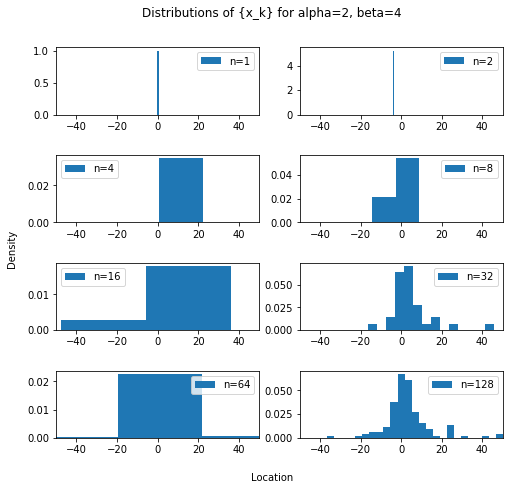
\includegraphics[width=.9\linewidth]{./obipy-resources/322vFv.png}

\begin{minted}[frame=lines,fontsize=\scriptsize]{python}
for i, mean in enumerate(new_means):
    print('n=%s, mean=%s'%(nvals[i], mean))
\end{minted}

\begin{verbatim}
n=1, mean=0.04
n=2, mean=-3.795
n=4, mean=25.0525
n=8, mean=-9.23
n=16, mean=-44.438750000000006
n=32, mean=2.180625000000001
n=64, mean=-38.13999999999999
n=128, mean=5.537265625
\end{verbatim}

Here in both cases we see that the mean is not really converging to the correct
value of alpha. This is because our distribution is not really bounded, and we
can get crazy high or low values which skew the data.

\subsection*{Total Log-Likelihood}
\label{sec-2-3}

Now, in calculating our likelihood, we'll just muliply the individual
probabilities of getting certain distances given alpha and beta together.

\begin{minted}[frame=lines,fontsize=\scriptsize]{python}
def get_log_likelihood(rounded_data, alpha, beta):
    log_like = np.sum(np.log(np.array(
        [get_prob(d, alpha, beta) for d in rounded_data])))
    return log_like
\end{minted}


For our prior we'll just choose a uniform distribution but with reasonable
bounds, i.e. alpha is between -10, 10, and beta is between 0, 10 (although in
this first example beta is known).

\begin{minted}[frame=lines,fontsize=\scriptsize]{python}
def get_posterior(data, alpha_val, beta_val, prior_func, **prior_kwargs):
    post = get_log_likelihood(data, alpha_val, beta_val) * prior_func(alpha_val)
    return post
\end{minted}

\subsection*{Plotting Posteriors over $\alpha$}
\label{sec-2-4}

\begin{minted}[frame=lines,fontsize=\scriptsize]{python}
def plot_alpha_posts(n, alpha, beta, ax):
    alpha_vals = np.linspace(-10, 10, 1000)
    locs = np.round(get_rand_locs(n, alpha, beta), 2)
    # start with beta = its real value
    post = [get_posterior(locs, a, beta, uniform_prior) for a in alpha_vals]
    # normalize to get max of 1, take 0th index
    post = np.array(post) / np.abs(np.max(post))
    # re-exponentiate
    post = np.exp(post)
    ax.plot(alpha_vals, post, label='n=%s'%n)
    prior_vals = np.array([1 for a in alpha_vals])
    normed_vals = prior_vals * (np.max(post) / np.max(prior_vals))
    ax.plot(alpha_vals, normed_vals, label='prior')
    ax.legend()
    max_ind = np.argmax(post)
    vals = np.array([[a, beta] for a in alpha_vals])
    return vals[max_ind]
\end{minted}


\begin{minted}[frame=lines,fontsize=\scriptsize]{python}
def plot_total_alpha_posts(alpha, beta):
    alpha_maxvals = []
    fig, axes = plt.subplots(4, 2, figsize=(8, 7))
    for i, n in enumerate(nvals):
        maxL = plot_alpha_posts(n, alpha, beta, axes.flatten()[i])
        alpha_maxvals.append(maxL)

    plt.suptitle('Posterior Distributions for real alpha=%s, beta=%s'%(alpha, beta))
    fig.text(0.5, 0.04, 'Alpha', ha='center')
    fig.text(0.04, 0.5, 'Posterior Density', va='center', rotation='vertical')
    plt.subplots_adjust(top=0.9, hspace=.6)
    plt.show()
    return alpha_maxvals
\end{minted}


\begin{minted}[frame=lines,fontsize=\scriptsize]{python}
alpha_maxvals = plot_total_alpha_posts(0, 2)
\end{minted}

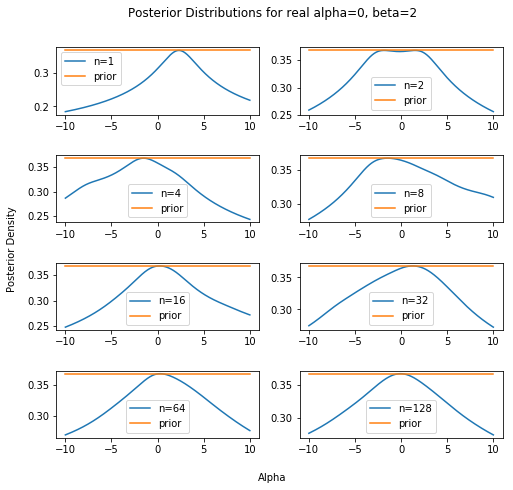
\includegraphics[width=.9\linewidth]{./obipy-resources/322i00.png}

\subsubsection*{Maximum Posterior Parameters}
\label{sec-2-4-1}

\begin{minted}[frame=lines,fontsize=\scriptsize]{python}
print('Maximum posterior parameters found with beta fixed:')
for i in range(len(alpha_maxvals)):
    print('n=%s, alpha=%s, beta=%s'%(nvals[i], alpha_maxvals[i][0], 
                                     alpha_maxvals[i][1]))
\end{minted}

\begin{verbatim}
Maximum posterior parameters found with beta fixed:
n=1, alpha=2.3123123123123115, beta=2.0
n=2, alpha=1.511511511511511, beta=2.0
n=4, alpha=-1.511511511511511, beta=2.0
n=8, alpha=-1.471471471471471, beta=2.0
n=16, alpha=0.21021021021021014, beta=2.0
n=32, alpha=1.2512512512512508, beta=2.0
n=64, alpha=0.2702702702702702, beta=2.0
n=128, alpha=-0.07007007007007005, beta=2.0
\end{verbatim}

Let's try with a different 'real' value of $\alpha$:

\begin{minted}[frame=lines,fontsize=\scriptsize]{python}
newalpha_maxvals = plot_total_alpha_posts(3, 4)
\end{minted}

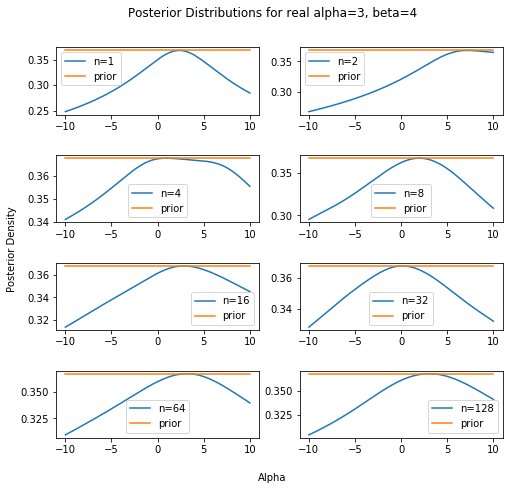
\includegraphics[width=.9\linewidth]{./obipy-resources/322uSQ.png}

\begin{minted}[frame=lines,fontsize=\scriptsize]{python}
print('Maximum posterior parameters found with beta fixed:')
for i in range(len(alpha_maxvals)):
    print('n=%s, alpha=%s, beta=%s'%(nvals[i], newalpha_maxvals[i][0], 
                                     newalpha_maxvals[i][1]))
\end{minted}

\begin{verbatim}
Maximum posterior parameters found with beta fixed:
n=1, alpha=2.3523523523523515, beta=4.0
n=2, alpha=7.217217217217218, beta=4.0
n=4, alpha=0.9509509509509506, beta=4.0
n=8, alpha=1.9719719719719713, beta=4.0
n=16, alpha=2.8528528528528536, beta=4.0
n=32, alpha=0.13013013013013008, beta=4.0
n=64, alpha=3.173173173173174, beta=4.0
n=128, alpha=3.0530530530530537, beta=4.0
\end{verbatim}

\subsection*{Posteriors Over $\alpha$ and $\beta$}
\label{sec-2-5}

Looks like this works pretty well! Now let's just do the same for a range of
beta values:

\begin{minted}[frame=lines,fontsize=\scriptsize]{python}
def plot_grid_posts(n, alpha, beta, ax):
    alpha_vals = np.linspace(-10, 10, 100)
    # start with beta = its real value
    beta_vals = np.linspace(0, 10, 100)
    locs = np.round(get_rand_locs(n, alpha, beta), 2)
    post = [[get_posterior(
        locs, a, b, uniform_prior) for a in alpha_vals] for b in beta_vals]
    # normalize to get max of 1, take 0th index
    post = np.array(post) / np.abs(np.max(post))
    # re-exponentiate
    post = np.exp(post)
    ax.contour(alpha_vals, beta_vals, post, 15)

    max_val = 0
    index = [0, 0]
    for i in range(len(post)):
        for j in range(len(post[i])):
            if (post[i][j] > max_val):
                max_val = post[i][j]
                index = [i, j]

    vals = np.array([[[a, b] for a in alpha_vals] for b in beta_vals])
    return vals[index[0]][index[1]]
\end{minted}


\begin{minted}[frame=lines,fontsize=\scriptsize]{python}
def plot_total_grid_posts(alpha, beta):
    total_maxLs = []
    fig, axes = plt.subplots(4, 2, figsize=(8, 7))
    for i, n in enumerate(nvals):
        maxLs = plot_grid_posts(n, alpha, beta, axes.flatten()[i])
        total_maxLs.append(maxLs)

    plt.suptitle('Posterior Distributions for real alpha=%s, beta=%s'%(alpha, beta))
    fig.text(0.5, 0.04, 'Alpha', ha='center')
    fig.text(0.04, 0.5, 'Posterior Density', va='center', rotation='vertical')
    plt.subplots_adjust(top=0.9, hspace=.6)
    plt.show()
    return total_maxLs
\end{minted}


\begin{minted}[frame=lines,fontsize=\scriptsize]{python}
maxLs = plot_total_grid_posts(0, 2)
\end{minted}

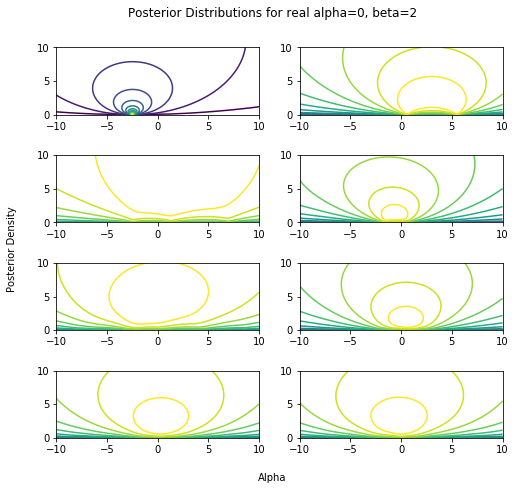
\includegraphics[width=.9\linewidth]{./obipy-resources/322uLc.png}


\begin{minted}[frame=lines,fontsize=\scriptsize]{python}
print('maximum posterior parameters found:')
for i in range(len(nvals)):
    print('n=%s, alpha=%s, beta=%s'%(nvals[i], maxLs[i][0], maxLs[i][1]))
\end{minted}

\begin{verbatim}
maximum posterior parameters found:
n=1, alpha=-2.525252525252525, beta=0.10101010101010101
n=2, alpha=3.5353535353535346, beta=2.4242424242424243
n=4, alpha=1.3131313131313131, beta=4.646464646464646
n=8, alpha=-0.7070707070707076, beta=1.0101010101010102
n=16, alpha=-0.7070707070707076, beta=3.131313131313131
n=32, alpha=0.5050505050505052, beta=1.2121212121212122
n=64, alpha=0.30303030303030276, beta=1.8181818181818181
n=128, alpha=-0.10101010101010033, beta=1.9191919191919191
\end{verbatim}

Now let's try with different alpha, beta:

\begin{minted}[frame=lines,fontsize=\scriptsize]{python}
new_maxLs = plot_total_grid_posts(3, 4)
\end{minted}

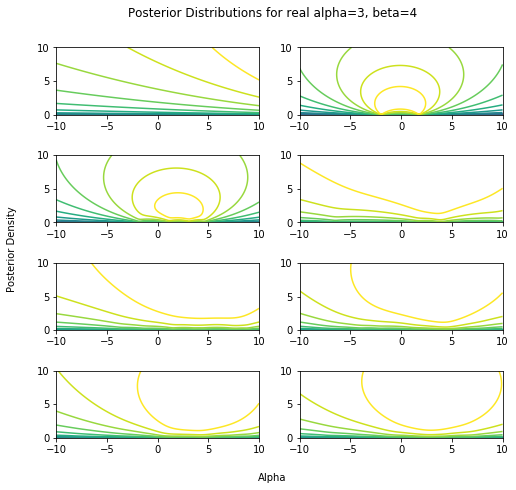
\includegraphics[width=.9\linewidth]{./obipy-resources/3227Vi.png}


\begin{minted}[frame=lines,fontsize=\scriptsize]{python}
for i in range(len(nvals)):
    print('n=%s, alpha=%s, beta=%s'%(nvals[i], new_maxLs[i][0], new_maxLs[i][1]))
\end{minted}

\begin{verbatim}
n=1, alpha=10.0, beta=10.0
n=2, alpha=-1.3131313131313131, beta=1.4141414141414141
n=4, alpha=2.525252525252524, beta=1.7171717171717171
n=8, alpha=2.525252525252524, beta=8.282828282828282
n=16, alpha=4.545454545454545, beta=6.262626262626262
n=32, alpha=3.333333333333334, beta=4.848484848484849
n=64, alpha=3.9393939393939394, beta=3.9393939393939394
n=128, alpha=3.1313131313131315, beta=4.242424242424242
\end{verbatim}

Here we see that alpha and beta are taking a lot longer to converge but are
eventually getting down to where we expect them.
% Emacs 25.2.1 (Org mode 8.2.10)
\end{document}
